\documentclass[11pt]{article}
\usepackage[margin=1in]{geometry}
\usepackage[T1]{fontenc}
\usepackage[utf8]{inputenc}
\usepackage{lmodern,microtype}
\usepackage{amsmath,amssymb,graphicx,booktabs,array}
\usepackage[round,authoryear]{natbib}
\usepackage{caption}
\usepackage{xcolor}
\usepackage[colorlinks=true,allcolors=blue,breaklinks=true]{hyperref}
\hypersetup{pdftitle={Evaluating fixed-kernel joint acquisition for cross-context perturbation prediction},pdfauthor={Abdullah Hamza}}
\captionsetup{font=small,labelfont=bf}
\setlength{\emergencystretch}{2em}
\setlength{\tabcolsep}{4pt}
\newcommand{\R}{\mathbb R}
\newcommand{\ForwardPercent}{0.5651}
\newcommand{\ForwardArea}{0.00786844}
\newcommand{\ForwardNoisePercent}{59.68}
\newcommand{\ForwardRank}{0.07931}
\newcommand{\ForwardCosine}{0.08719}
\newcommand{\ReversePercent}{0.01378}
\newcommand{\ReverseArea}{0.00572383}
\newcommand{\ReverseNoisePercent}{79.40}
\newcommand{\ReverseRank}{0.03856}
\newcommand{\ReverseCosine}{0.02784}

\title{Evaluating fixed-kernel joint acquisition for cross-context perturbation prediction}
\author{Abdullah Hamza\\Independent Researcher\\\href{mailto:abdullah2hamza@gmail.com}{\texttt{abdullah2hamza@gmail.com}}}
\date{October 23, 2026}
\begin{document}
\maketitle
\begin{abstract}
Predicting an intervention's response in a new context can require choosing which other interventions to measure, how many cells to acquire, and how much to spend on shared controls. We evaluate a fixed radial-basis-function discrepancy-variance augmentation of greedy worst-query design under this joint budget. A finite-pool replay separates supplied source responses, paid recipient calibration cells and sealed recipient assessment cells; all policies share prediction backbones and explicit purchase ledgers. In a frozen K562/RPE1 replay with 131 held-out interventions, rank-four source coordinates and budgets 128--512, the augmentation changes paid-validation ridge error area by $+0.565\%$ and $+0.0138\%$ in the two directions, respectively; conditional query-resampling ranges include zero. The pilot already spans the estimated representation, and assessment noise is large relative to prediction gains. A separately declared post-primary study crosses two new split/cell-order seeds, ranks 4/16 and budgets through 2,048. Six of eight wider-grid point contrasts favor worst-query, while five favor the extension against mean-query. One forward rank-four cell improves by $3.58\%$ against worst-query, demonstrating sensitivity rather than a universal negative result. Known-truth experiments expose a further failure: noisy source coordinates can make a missing direction appear supported, while ideal Gaussian intervals miss structural error. These findings concern one fixed acquisition surrogate, whose variance is not the fitted ridge predictor's risk. The contribution is an auditable evaluation of its limitations and conditional successes, with complete comparisons, uncertainty scopes and reproducible artifacts; it does not establish biological transportability or prospective laboratory savings.
\end{abstract}
\noindent\textbf{Keywords:} perturbation prediction; experimental design; shared controls; transfer learning; computational reproducibility
\section{Introduction}
Perturbation atlases measure selected interventions in selected cellular contexts, leaving most intervention--context combinations unobserved. Genome-scale Perturb-seq and multimodal perturbation screens provide unusually rich settings for studying this missingness \citep{replogle2022,frangieh2021}, while harmonized releases make computational replay practical \citep{scperturb2024}. We consider a particular information interface: the response to each query intervention has been measured in a supplied source context, but its recipient response remains unavailable. A limited recipient budget can purchase responses to other calibration interventions and additional controls. The choice is not only which interventions to measure, but how deeply to measure each one and how much to spend on the shared control reference.

These choices couple prediction, measurement precision and transfer assumptions. Another calibration intervention can improve coverage of source-response directions; more cells reduce sampling noise; more shared controls improve all control-relative contrasts together. However, a well-conditioned fit in estimated source coordinates can coexist with misspecified transfer or errors in those coordinates. A design criterion that reduces a surrogate variance need not improve a strongly regularized predictor's squared error. Distinguishing these possibilities requires matching information, prediction backbones and actual purchases, rather than comparing method names with different access to recipient labels.

The constituent ideas have substantial precedent. IterPert uses multimodal and cross-context priors for sequential perturbation acquisition \citep{iterpert2024}. PerturbPlan studies prospective power/cost trade-offs involving cell and read depth \citep{perturbplan2026}; its association-testing objective differs from sealed-query response prediction. PerturbMap transports the same intervention's source response through calibrated cross-context experts \citep{perturbmap2026}. Shared-response references, gene-coordinate permutation and representation-coverage diagnostics have precedent in AmbiModBench \citep{ambimodbench2026}; we use related checks to qualify a different, costed acquisition estimand. Transductive experimental design separates measurement and query sets \citep{fiez2019}, and kernel posterior variance is classical \citep{gpml2006}. We claim neither priority for these components nor reproduction of the cited methods' published performance. Our comparators are specified implementations under one common replay interface; the transfer reconstruction's differences are disclosed.

Our empirical question is narrower: does adding a fixed source-coordinate radial-basis-function (RBF) discrepancy-variance term to a covariance-aware greedy worst-query design improve a shared paid-validation ridge predictor? The added term is a concrete hypothesis, not an estimator of realized structural bias or a fitted discrepancy component of the prediction model. We test it in known-truth simulations, a separate development context, and a frozen bidirectional released-data replay. Post-primary analyses and a separately declared split/rank/budget robustness study examine limitations without replacing the original comparison.

The contribution is a precisely specified, reproducible evaluation with negative and failure evidence. We expose the roles of shrinkage, shared controls, estimated support and evaluation noise; preserve complete crossed baselines and paid ledgers; and distinguish absolute-effect error from ordinal ranking. The real-data evidence concerns a count-selected cohort and dependent replay tasks, not independent biological replications or prospective laboratory savings. In particular, the original real pilot already spans the estimated rank-four representation: those runs principally test precision allocation conditional on estimated support, rather than an identification transition.

\section{Task, estimand and methods}
\label{sec:methods}
\subsection{Information, finite pools and costs}
Let $\mathcal C$ be eligible recipient calibration interventions and $\mathcal Q$ a disjoint, fixed query set, grouped by canonical target gene so guides cannot cross the split. Source responses for both sets are supplied. A policy sees source summaries and only recipient cells already purchased through a finite-pool service. Its actions open a calibration intervention, add cells to an opened intervention, or add shared negative-control cells. It cannot purchase query outcomes. An append-only ledger records cell identifiers, action costs and cumulative spend; previously purchased cells cannot be reused within a ledger.

Each policy has its own counterfactual paid ledger. The same policy seed gives matched pilot identities and the same per-condition cell order across policies. Setup costs four abstract units per opened intervention; perturbed and control cells each cost one. The pilot buys six interventions at eight cells each and 16 controls, totaling 88. Subsequent blocks contain eight cells; affordable partial blocks are allowed, with at least two cells required to open an intervention. Unaffordable actions stop acquisition, and actual spend is reported. The units are hypothetical: a pooled screen does not inherently permit purchasing an arbitrary chosen gene's next cells. Real implementation could require enrichment, reweighting or arrayed experiments.

Independent scorer-only treatment/control banks are inaccessible to the policy and predictor. For the primary external suite, all six runs close and authenticate their predictions before any scorer opens. This joint barrier protects the intended cooperative workflow; it is not a security sandbox against a hostile process with filesystem access. Source observations and scorer resources are disclosed separately from predictor-used recipient costs. Selecting a null predictor does not refund its acquisition policy's paid observations; a standalone zero predictor has zero recipient measurement-use cost.

\subsection{Expression target and source coordinates}
For a count vector $c$, preprocessing applies
\begin{equation}
 T_g(c)=\log\!\left(1+10^4c_g/\sum_{h\in\mathcal G_{\rm released}}c_h\right).
\end{equation}
The population target is $\delta_{ig}=E[T_g(c)\mid i]-E[T_g(c)\mid 0]$ in the recipient, estimated for scoring by independent treatment/control cell means. It is a difference of normalized-log means, not a count-mean log fold change. Each file's complete released panel enters normalization before the exact source/recipient gene intersection. Different released panels therefore define different compositional denominators.

Center the supplied source-response matrix over interventions and obtain its leading $r$ principal coordinates through its intervention Gram matrix. Scale the coordinates to unit root-mean-square and append an intercept, producing $x_i\in\mathbb R^{r+1}$, including coordinates $q_i$ for source-observed queries. This is transductive access to \emph{source} query responses, not recipient query labels. The primary external representation fixes $r=4$. Source half-sample differences and variance estimates are diagnostic inputs; they are not fully propagated into fitted uncertainty.

\subsection{Shared controls, regularization and support}
Under an ideal linear response model $\delta_i=x_i^\top B$, let treatment-mean noise variance be $d_i=v_i/n_i$ and control-mean variance be $c=v_0/n_0$. Let $\mathcal A(s)=\{i\in\mathcal C:n_i(s)>0\}$ denote the currently purchased calibration identities, and $X=X_{\mathcal A}$, $Y=Y_{\mathcal A}$ their rows. For a single expression coordinate, their observed control-relative effects have covariance
\begin{equation}
 C=\operatorname{diag}(d_i)+c\mathbf 1\mathbf 1^\top,
 \qquad M=X^\top C^{-1}X.
 \label{eq:cov}
\end{equation}
The implementation evaluates the equivalent weighted centered scatter including a zero-feature control group and uses a factored generalized least-squares solve, avoiding unstable subtraction. Scalar variances average measurement variability over expression genes. Opened interventions use purchased-cell estimates; unopened interventions use source variance multiplied by the median recipient/source ratio learned from paid observations. This is a plug-in working model, not a complete gene-specific or batch-dependent noise model.

For positive control depth, a query is linearly estimable under the fixed-feature model only when $q$ lies in the row space of $X$ (equivalently the range of $M$). We compute projection residuals before ridge and assign unsupported queries infinite ideal variance. A relative eigenvalue tolerance $10^{-9}$ defines numerical support. Regularizing $M$ makes a point fit unique but does not establish identification from observations. Errors in estimated source coordinates or misspecified transfer can invalidate even a full numerical support diagnosis (Appendix~\ref{app:math}). This is linear-model algebra, not identification of biological transportability.

The principal prediction backbone solves
\begin{equation}
 \widehat B_\lambda=\arg\min_B\operatorname{tr}[(Y-XB)^\top C^{-1}(Y-XB)]+\lambda\|B\|_F^2.
\end{equation}
Paid leave-one-intervention-out validation selects among $\lambda\in\{.1,1,10,100,10^3,10^4,10^5\}$ and an explicit zero-effect candidate. For linear held-out prediction $a^\top Y_{-i}$, its score subtracts the held-out mean variance and shared-control variance and adds $2c\sum_j a_j$. Under fixed design and known variances this corrects shared-control validation covariance; the derivation and limitations appear in Appendix~\ref{app:math}. Plug-in variances, adaptivity and winner selection preclude an end-to-end unbiased-risk guarantee.

\subsection{The evaluated acquisition augmentation}
Let $V_{\max}=\max_{q\in\mathcal Q}q^\top(M+.01I)^{-1}q$. The classical worst-query rule greedily selects an affordable action's reduction in $V_{\max}$ per cost. The mean-query rule replaces the maximum by an average, aligning its ideal variance objective more closely with mean squared error. Both are greedy working-model rules, not global optimizers of realized prediction loss.

The evaluated extension adds a fixed kernel-variance term. For non-intercept standardized source coordinates $z_i\in\mathbb R^r$, set
\begin{align}
 K_{ij}&=\exp[-\|z_i-z_j\|^2/(2r\ell^2)],\\
 V_K&=|\mathcal Q|^{-1}\operatorname{tr}\{K_{QQ}-K_{Q\mathcal A}(K_{\mathcal A\mathcal A}+C_{\rm noise}+10^{-6}I)^{-1}K_{\mathcal A Q}\}.
\end{align}
Here $C_{\rm noise}=\operatorname{diag}(v_i/n_i)_{i\in\mathcal A}+(v_0/n_0)\mathbf1\mathbf1^\top$ conditions on purchased interventions only; an empty set gives the prior query variance. The kernel is unit amplitude, $\ell=1$, and $C_{\rm noise}$ includes shared-control covariance. The covariance expression is standard Gaussian-process algebra \citep{gpml2006}; here it treats the linear trend as known. For state $s$ and action $a$, the actual extension score is
\begin{equation}
 U(a)=\frac{V_{\max}(s)-V_{\max}(s+a)+\gamma[V_K(s)-V_K(s+a)]+10^6 H(s,a)}{\operatorname{cost}(a)},
 \label{eq:acquisition}
\end{equation}
where $H$ is the nonnegative decrease in summed query projection-residual fractions while any query is unsupported, and is zero once all are supported. The finite support bonus is also used by the query-directed classical rules. Setting $\gamma=0$ reproduces worst-query acquisition. Development selected $\gamma=1$; the original $.25$ is retained as a comparator.

Crucially, the kernel term's amplitude is not learned from realized residual bias, and the fitted primary predictor does not include this GP discrepancy. Its variance is therefore not the primary ridge predictor's risk. Evidence about Equation~\ref{eq:acquisition} cannot reject bias-aware acquisition generally or establish online detection of mechanism shift.

\subsection{Matched predictors, policies and controls}
Each policy's identical purchases feed zero effect, shared mean, source copy, scalar affine transfer, fixed-ridge GLS, paid-validation ridge, heuristic local residual adaptation, a recipient-local low-rank network and a single-source PerturbMap-style reconstruction. The last two share a training-only rank-16 response basis, paid-control descriptors, a 128-unit LayerNorm/GELU network and fixed model seed; they are not author-code reproductions. Appendix~\ref{app:implementation} specifies optimization and fidelity differences. Early stopping, transport selection and interpolation reuse the paid validation set, so the reconstruction's fitted calibration improvement is not an independent reliability test.

The original external suite includes random/equal allocation, a development-selected fixed grid, source diversity, D-optimal, worst-query, mean-query, reliability and disagreement rules alongside the extension. Six allocation/covariance/extension ablations and the original discrepancy weight are retained. Source-identity derangement and query-source gene-coordinate permutation are run in both directions with fixed permutations and four prespecified policies. The corrupted public sources are processed through the same source-only coordinate pipeline. Scoring-coordinate permutation is a separate post-primary diagnostic without refitting. Every comparison retains its information, cost and task qualification.

\section{Study design and analysis}
\label{sec:experiments}
\subsection{Public data and selected population}
We pin the scPerturb version-1.4 release (Zenodo record 13350497) \citep{scperturbdata,scperturb2024}, verify published checksums and retain SHA-256 provenance. The Frangieh RNA dataset supplies development from the environment labelled Control to IFN$\gamma$ stimulation \citep{frangieh2021}; it is not pooled with the external CRISPRi data. Development restricts multiplicity of infection to one, retains at most 96 cells per intervention/context and 512 negative controls, and uses 205 eligible target identities (154 calibration, 51 query) and 23,712 expression genes. Source eligibility permits at least 32 cells, while recipient banks require 64 acquisition and 32 assessment cells. Development observations that inform tuning, including scorer-only outcomes once used for selection, are charged in a separate unique-exposure union.

The external pair comprises Replogle K562-essential and RPE1 RNA releases \citep{replogle2022}. Of 2,057 and 2,393 released non-control target labels, respectively, 525 have at least 96 cells in both files and matching canonical target identifiers. Thus the evaluated cohort represents approximately 25.5\% and 21.9\% of those label inventories; it is not a random sample of all genes. A metadata-defined split reserves 131 queries and 394 calibration candidates. Exact expression-gene alignment leaves 7,226 genes from panels of 8,563 and 8,749. Each supplied source uses 96 cells per target plus 512 controls (50,912 cells). Recipient calibration pools contain 64 cells per intervention; each query has 32 scorer-only cells, with 256 acquisition and 256 independent assessment controls. Each direction's scorer uses 4,448 cells.

Paired guides in Replogle target one gene. Canonical annotation and guide-ownership audits prevent target/guide leakage across the split. No donor or independent biological-replicate field is available. K562 essential was profiled at day 6 with dCas9-KRAB, versus RPE1 at day 7 with a ZIM3-derived effector. Together with differing normalization panels and survival/capture selection, these differences make the task combined biological/protocol transfer, not an isolated cell-line effect. Count-uniform public pools do not remove selection of the count-eligible cohort. Both directions reuse target identities and cells in different roles: cells used for assessment in one direction may contribute to supplied source summaries in the other. Run-specific objects and permitted inputs remain isolated; the directions are not independent blinded biological datasets.

\subsection{Development and the frozen primary test}
Initial five-seed pilots and a 70-case controlled study preceded final external scoring. A predeclared development grid compared nine fixed allocation grids and five discrepancy weights, selecting control fraction $.125$, depth 8 and weight $\gamma=1$ at length one. The full final development exposure is 6,428 abstract units. This historical fixed charge is reported separately from external incremental budgets and from the supplied source atlas. It is not an experimentally verified total laboratory-program price.

The original external configuration fixes budgets 128/256/512, source rank four, acquisition seeds 0--4, nine prediction backbones and all main policies/ablations. Two unmodified 16-policy runs and four four-policy permutation runs yield 720 checkpoints and 848,880 query/backbone metric rows. Every run's predictions close before the first scorer access, with immutable configuration, episode, source and ledger-prefix bindings. These engineering checks support the information-interface claim; they do not validate transfer assumptions.

The five primary seeds vary pilot identity order and policy tie choices on one fixed split and fixed per-condition cell order. They do not resample cells or vary neural initialization. The primary contrast is extension minus worst-query acquisition with the same paid-validation ridge predictor. For budget $b$, define
\begin{align}
 E(b)&=\frac{1}{|\mathcal Q|SG}\sum_{i\in\mathcal Q}\sum_{s=1}^{S}\sum_{g=1}^{G}
 (\widehat\delta_{isg}(b)-\widetilde\delta_{ig})^2,\notag\\
 A&=\frac{\sum_{j=1}^{J-1}(b_{j+1}-b_j)[E(b_j)+E(b_{j+1})]/2}{b_J-b_1}.
 \label{eq:endpoint}
\end{align}
Here $\widetilde\delta$ is the independent assessment contrast, $S=5$ and $J=3$ in the primary external test. There is no observation below the first budget. Negative paired area differences favor the extension. The primary endpoint averages the entire aligned expression panel without selecting genes from recipient query effects.

The prospective research dossier originally suggested the strongest development-selected baseline. The actual final pre-scoring freeze instead selected worst-query to isolate the added component. We disclose this change: it does not establish that worst-query is the best design, and its maximum-variance objective differs from the mean-error endpoint. Mean-query and the full crossed comparisons are retained. Post-primary references to development's strongest overall point estimate (zero) and strongest paid combination (reliability/CV ridge) do not replace the primary test or become confirmatory discoveries.

\subsection{Uncertainty and supplementary diagnostics}
We average acquisition seeds within each query before a descriptive query bootstrap (2,000 draws, seed 20261022). Its central 95\% resampling range fixes source, split, fitted predictions and scorer bank; it is not a biological confidence interval. Separate fixed-query cell resampling preserves one shared control resample across queries. A guide/batch-stratified version preserves the observed mixture, while common technical-batch exponential weights provide a different sensitivity analysis. We never pool these ranges into a combined interval or count genes, seeds, splits or reused directions as independent biological replicates. The paired-error projection and analytic variance check are detailed in Appendix~\ref{app:math}.

Scorer noise floors use within-bank cell variances and independent-cell mean-variance formulas. They provide plug-in scale context, not known population truth or protection against shared batch dependence. Noise-subtracted errors are not clipped. Numerical 90/95\% Gaussian widths use unregularized ideal variance around fixed-ridge predictions; real compatibility additionally includes assessment noise. They deliberately omit regularization bias, source error, adaptivity and misspecification. We use their failures diagnostically, not as a calibrated uncertainty method.

Post-primary scoring of frozen predictions includes sign agreement with explicit zero ties; raw direction and centered response-specific cosine; within-query gene correlation; and gene-wise Spearman ranks \emph{across query identities}. Constant genes have undefined Spearman correlation and reported denominators. A separately labelled fixed-gene score assigns undefined terms neutral zero. A per-gene control shift preserves ranks, which does not validate absolute effects. Scoring-gene permutation uses seed 20261022 without refitting. Source-warning, estimated-support, variance and nearest-paid-source-distance retention use label-free thresholds/ties and full query/seed denominators. No observed query error chooses a retention cutoff.

\subsection{Controlled and post-primary robustness studies}
The original known-truth simulation uses 24 interventions, 64 expression coordinates, three latent directions, 32 source cells per intervention, 24 recipient acquisition and assessment cells per intervention, and 64 controls in each independent bank. Six queries and 18 calibration identities are split independently of latent generation. Fourteen scenarios separate source feature/measurement error, recipient/control noise, nonlinear shift, missing calibration directions, shared batch offsets and source permutations. Five independent generative seeds 71--75 are reused across scenarios as common random draws; five acquisition seeds are averaged within each world before paired world-level Monte Carlo standard errors. Scenario counts are not replication. Budgets are 96/144/192 and the discrepancy weight is the original $.25$. Oracle support and true effects enter only the post-prediction scorer.

Separately declared after the primary results, 30 price-sensitivity cases cross setup/cell ratios 0/16/64, baseline/nonlinear scenarios and five new generative seeds 171--175 at budgets 512/768/1,024. These worlds recur across prices/scenarios. A combined identity-only ablation freezes depth/controls after the pilot. Finite-pool exhaustion and constrained underspend are reported, not interpreted as equal-expenditure superiority.

PI review additionally requested the post-primary robustness matrix in Table~\ref{tab:study}. Two new episode seeds (20261023/20261024) change query membership and within-condition cell order/banks, and both directions are crossed with ranks 4/16 and budgets 128/256/512/1,024/2,048. Worst-query, mean-query and the unchanged extension share all seven legacy backbones and three acquisition-order/tie seeds. The eight-run suite closes 360 checkpoints jointly before new scoring. This challenges the original full-support, small-budget regime; it uses reused public data and is not renewed external confirmation. Settings and every matrix cell are retained regardless of sign.

A final descriptive influence analysis of original saved outputs reports paired query contributions, all leave-one-query-out mean shifts, seed variation and the originally frozen public-source strata. It excludes no query. Direct query measurement is a separate stronger-information task using reserved query cells with its own paid ledgers and disjoint scorer banks; it is not a primary-task competitor or an optimized estimator over every possible direct-information procedure.

\section{Original frozen results}
\label{sec:results}
\subsection{No demonstrated primary benefit, with limited predictive signal}
Table~\ref{tab:primary} and Figure~\ref{fig:primary} give the frozen component comparison. The extension's paid-validation ridge area is slightly higher in both directions: $+0.5651\%$ K562 to RPE1 and $+0.0138\%$ RPE1 to K562. Both conditional query-resampling ranges cross zero. These observations show no demonstrated advantage in this replay; they neither establish equivalence nor rule out benefits under other splits, representations or budgets.

\begin{table}[htbp]
\centering\small
\caption{Frozen primary comparison. $A_E$ and $A_W$ are normalized MSE areas for the extension and worst-query, in units of $10^{-3}$. Difference $\Delta=A_E-A_W$ and its central 95\% conditional query-resampling range use units of $10^{-5}$. Positive values favor worst-query. Five acquisition-order/tie seeds share one fixed cell bank.}
\label{tab:primary}
\begin{tabular}{lrrrrr}
\toprule
Direction & $A_E$ & $A_W$ & $\Delta$ & Query range & Change (\%) \\
\midrule
K562$\to$RPE1 & 7.86844 & 7.82422 & +4.4212 & [-4.4957, +13.0315] & +0.5651 \\
RPE1$\to$K562 & 5.72383 & 5.72305 & +0.0789 & [-0.4150, +0.5948] & +0.0138 \\
\bottomrule
\end{tabular}

\end{table}

\begin{figure}[htbp]
\centering
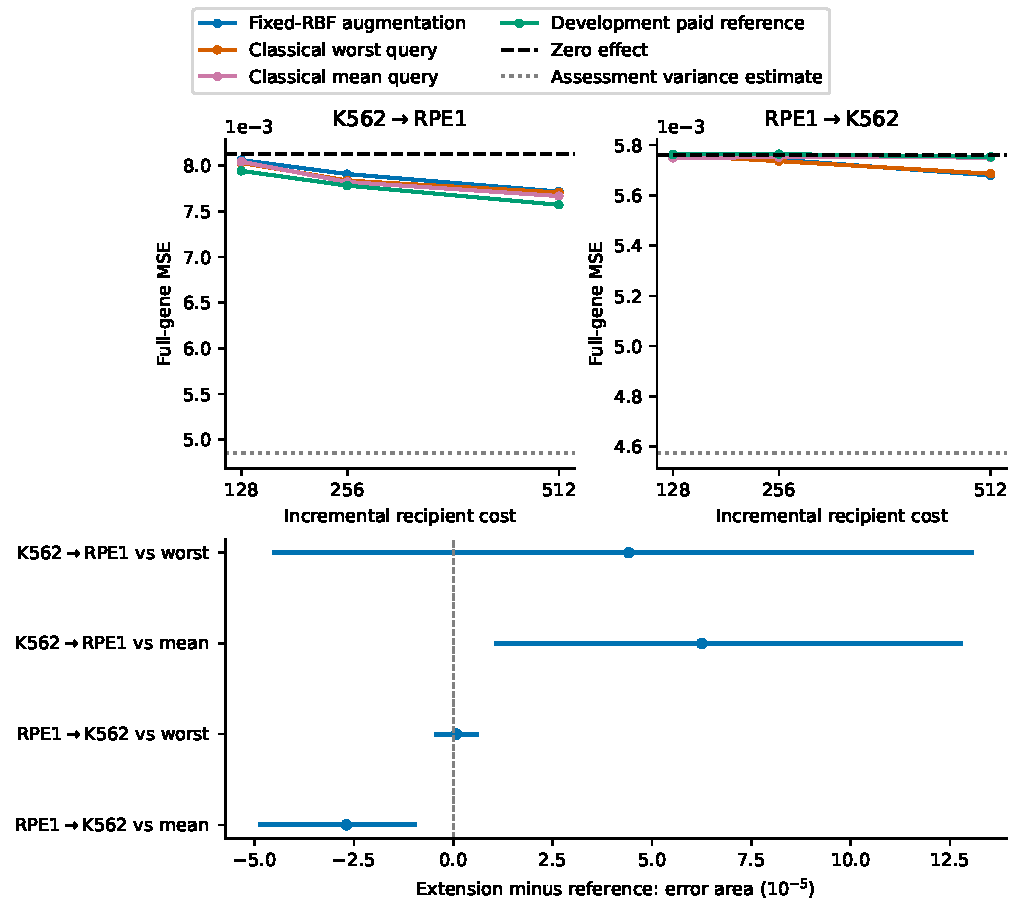
\includegraphics[width=\linewidth]{figures/primary-results.pdf}
\caption{Original real-data replay. Upper panels show observed MSE against abstract incremental recipient budget. Zero is a standalone zero-recipient-cost reference; its horizontal placement does not charge it the displayed purchases. The estimated assessment noise floor is plug-in context, not a known lower bound under arbitrary dependence. Lower panels show paired error-area differences and conditional query-resampling ranges, with all acquisition seeds averaged within query. Mean-query and worst-query use the same paid-validation ridge predictor. Development-selected reliability is a post-primary reference. Directions reuse observations; the ranges are not biological confidence intervals.}
\label{fig:primary}
\end{figure}

Comparator choice matters. Against mean-query, the extension changes area by $+0.8015\%$ forward and $-0.4678\%$ reverse, with conditional query ranges wholly above and below zero, respectively. Table~\ref{tab:devrefs} adds the development-selected references. The extension is $1.694\%$ worse than reliability/CV ridge forward and $0.623\%$ better reverse, with the latter range crossing zero. These post-primary comparisons cannot retrospectively replace the frozen hypothesis.

\begin{table}[htbp]
\centering\small
\caption{Post-primary comparisons with development-selected references. Differences and query ranges have units $10^{-5}$; negative changes favor the extension. Development's strongest overall point estimate was zero; reliability/CV ridge was its strongest paid combination. These are not new confirmatory tests.}
\label{tab:devrefs}
\begin{tabular}{llrrr}
\toprule
Direction & Development reference & Change (\%) & $\Delta$ & Query range \\
\midrule
K562$\to$RPE1 & Zero & -3.159 & -25.665 & [-47.096, -7.991] \\
K562$\to$RPE1 & Reliability/CV ridge & +1.694 & +13.106 & [+3.691, +23.889] \\
RPE1$\to$K562 & Zero & -0.623 & -3.590 & [-7.096, -0.774] \\
RPE1$\to$K562 & Reliability/CV ridge & -0.623 & -3.587 & [-8.563, +0.231] \\
\bottomrule
\end{tabular}

\end{table}

Observed zero-predictor areas are $.00812508$ and $.00575973$. The corresponding estimated scorer noise areas are $.00484897$ and $.00457337$, about $59.68\%$ and $79.40\%$ of zero error. Extension/ridge improves observed error over zero by only $3.159\%$ and $.623\%$. At budget 512 its gene-wise rank scores are $.07931$ and $.03856$, and raw direction cosines are $.08719$ and $.02784$. These weak scores and high measurement noise constrain biological interpretation. Noise subtraction is descriptive and does not turn a conditional resampling range into a population inference.

\subsection{Support, heterogeneity and source diagnostics}
An independent source-only audit finds rank five for all ten direction/seed pilot designs (four coordinates plus intercept), with all 131 query vectors in their estimated span. All 160 original policy trajectories share the same pilot prefix within direction/seed. Thus the original primary study tests precision allocation and shrinkage after estimated support, rather than recovery of an initially missing direction. The first 88 units are already spent before the budget-128 endpoint.

The paired-query distributions are heterogeneous (Figure~\ref{fig:influence}). Forward, 106/131 query-averaged differences favor worst-query and 25 favor the extension. Deleting any one query leaves the mean difference positive, ranging from $2.60\times10^{-5}$ to $7.13\times10^{-5}$. Reverse, 59 queries favor worst-query and 72 favor the extension; one leave-one-query-out deletion reverses the tiny positive aggregate. Individual acquisition-seed mean differences range from $-4.34\times10^{-5}$ to $1.82\times10^{-4}$ forward and $-2.20\times10^{-5}$ to $3.65\times10^{-5}$ reverse. These are dependence-aware descriptions, not independent seed replications. No query was excluded or used to choose a threshold.

\begin{figure}[htbp]
\centering
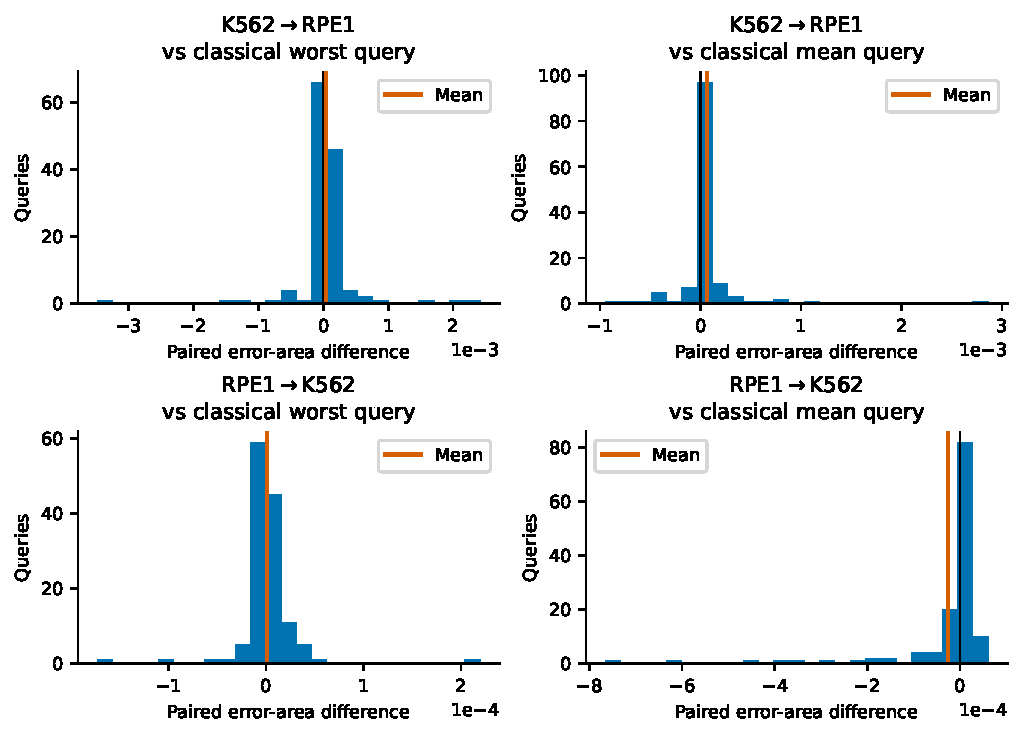
\includegraphics[width=\linewidth]{figures/query-contributions.pdf}
\caption{All 131 original paired query contributions per direction/reference, after averaging the five acquisition seeds. Negative values favor the extension. Orange lines mark means; they can differ from the median or majority sign. Histograms expose heterogeneity without changing the prespecified all-query endpoint. Queries share source estimation and assessment controls.}
\label{fig:influence}
\end{figure}

Source-warning heuristics flag 113/131 forward and 88/131 reverse queries. Retaining only unflagged queries would retain just 18 and 43, respectively, and can select harder queries rather than guarantee lower error. The original strong/weak-source strata and all retention denominators remain available; weak source response does not prove a null recipient effect. Source-identity permutation moves extension/ridge areas to $.00812767/.00576257$; query-source gene permutation gives $.00805871/.00576258$. These controls weaken intervention-specific transfer, but global offsets and shrinkage can survive corruption. Source-half sensitivity and support checks are diagnostics, not calibrated certificates.

Ordinal and absolute accuracy also differ. The reconstructed transport comparator has worse absolute-error area than the local network under all 16 policies in each direction, yet some centered specificity/rank metrics improve. Source copy has reverse rank score $.06820$, exceeding paid ridge's $.03856$ despite much worse absolute error. Table~\ref{tab:ranking} reports common denominators. These observations do not reproduce or refute PerturbMap's published result under its different implementation and task.

\subsection{Known-truth failures and conditional successes}
Across the 14 original controlled scenarios, the extension's true-error area is higher than worst-query in ten and lower in four. The baseline change is $+1.41\%$, while the nonlinear-shift case improves by $5.08\%$; all world-level uncertainties and scenarios are retained in Table~\ref{tab:all-scenarios}. Five generated worlds supply the independent Monte Carlo units, and scenarios reuse those worlds. In all 25 matched baseline/nonlinear world/acquisition-seed pairs, allocation sequences are identical. Hence the nonlinear improvement is conditional alignment of a fixed geometry-based allocation with a changed error surface, not detection of nonlinear bias. All 350 zero-weight/worst-query ledger pairs are byte-identical, verifying the component ablation.

Figure~\ref{fig:failures} illustrates a support counterexample. With an exact missing source direction, all 150 query/seed records are correctly unsupported; after source-coordinate error, all 150 appear estimated-supported while none is oracle-supported. This is a constructed failure, not an estimate of its prevalence in real screens. The same distinction affects uncertainty: for fixed ridge/worst-query at budget 192, nominal 95\% coverage is $.954$ in the baseline, $.864$ under nonlinear shift and $.781$ under source-feature error of standard deviation one. Widths fail to track the added structural error. These idealized Gaussian diagnostics are not a proposed valid adaptive inference method.

\begin{figure}[htbp]
\centering
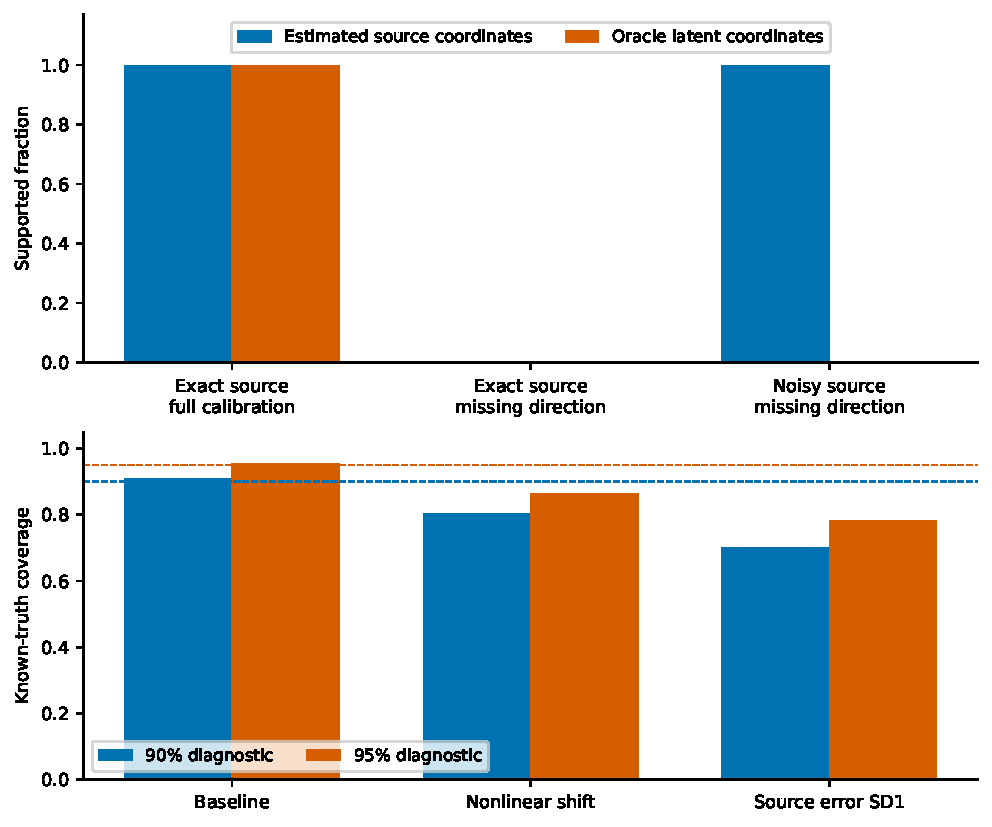
\includegraphics[width=\linewidth]{figures/support-and-coverage.pdf}
\caption{Known-truth support and coverage diagnostics. Upper panel: estimated versus oracle support for six queries across five acquisition seeds and five worlds at the final budget; 150 records are dependent observations, not independent worlds. Source-coordinate error can conceal a missing direction. Lower panel: empirical coordinate coverage of nominal 90/95\% intervals centered on fixed-ridge predictions, conditional on finite width. Baseline, nonlinear-shift and source-error settings separate sampling variance from omitted structural error. Complete widths and undefined counts appear in Table~\ref{tab:intervals}.}
\label{fig:failures}
\end{figure}

Price sensitivity and direct query measurement are supplementary (Appendix~\ref{app:assessment}). They do not establish real monetary savings or a universal budget boundary.

\section{Post-primary split, rank and budget sensitivity}
\label{sec:robustness}
\begin{table}[htbp]
\centering\small
\caption{Study stages and their evidential roles. Acquisition seeds vary order/ties unless cell-order variation is explicitly stated. Reused data/worlds do not supply independent biological replication.}
\label{tab:study}
\begin{tabular}{>{\raggedright\arraybackslash}p{.19\linewidth}>{\raggedright\arraybackslash}p{.35\linewidth}>{\raggedright\arraybackslash}p{.36\linewidth}}
\toprule
Stage & Scope & Role and timing\\
\midrule
Controlled & 14 scenarios, five worlds, five acquisition seeds; 96--192 & Known truth and failures; original settings, reused worlds\\
Development & Frangieh Control to IFN$\gamma$; 205 targets & Grid/weight selection; separate 6,428-unit exposure\\
Frozen primary & Both K562/RPE1 directions; one split, rank 4; 128--512; five seeds & Pre-scoring component comparison; fixed cell banks\\
Secondary & Prices 0/16/64; ranking, resampling, direct queries & Declared post-primary diagnostics; distinct information/cost scopes\\
PI robustness & Two new split/cell-order seeds; both directions; ranks 4/16; 128--2,048; three seeds & Post-primary sensitivity; all eight cells retained, data reused\\
\bottomrule
\end{tabular}
\end{table}

All eight additional runs completed, yielding 360 jointly closed checkpoints, 72 paid ledgers and 330,120 metric rows. Every policy/checkpoint reaches its exact budget ceiling. Figure~\ref{fig:robustness} shows all 32 extension contrasts: two query-design references and two budget grids per matrix cell. Tables~\ref{tab:robust-full} and \ref{tab:robust-original} retain absolute differences and conditional query ranges. The shorter grid reuses these new predictions at 128/256/512; it is not a new execution of the original fixed split.

On the full 128--2,048 grid, six of eight point contrasts favor worst-query and two favor the extension. Against mean-query the extension instead improves in five of eight cells. For split 20261023, forward rank four improves by $3.581\%$ versus worst-query ($\Delta=-.000301735$, conditional query range $[-.000570608,-.000051932]$) and $7.215\%$ versus mean-query. The benefit is already present on this split's shorter grid ($-3.435\%$ versus worst-query); extending the budget cannot be identified as its cause. For split 20261024, both forward ranks worsen versus worst-query. At reverse rank 16, split 20261023 changes from $-.100\%$ on the shorter grid to $+.308\%$ on the full grid. A blanket negative conclusion would conceal these changes.

The favorable full-grid aggregate is heterogeneous: only 47/131 query-averaged differences favor the extension versus worst-query, with median $+.000136211$. Deleting any one query leaves the mean negative, between $-.000331337$ and $-.000234779$. Thus the mean benefit is not a uniform query-level benefit or a single-query sign artifact. All 32 contrasts have retained deletion diagnostics, with no query excluded.

Table~\ref{tab:robust-absolute} places these contrasts beside zero and both design references. Rank-four full-grid error reductions versus zero are $10.485\%$ and $7.635\%$ forward, and $2.355\%$ and $2.098\%$ reverse. These larger gains differ from the original low-budget replay; new-grid direction/rank or prospective biological utility has not been established by these squared-error improvements.

\begin{table}[htbp]
\centering\footnotesize
\caption{Full-grid absolute error areas in units $10^{-3}$, including zero $A_0$ and the extension $A_E$, worst-query $A_W$ and mean-query $A_M$ with the same paid-validation ridge predictor. The last column compares the extension with zero. Split abbreviations match Table~\ref{tab:robust-full}. Zero is a standalone zero-recipient-cost prediction reference.}
\label{tab:robust-absolute}
\begin{tabular}{lrrrrrrr}
\toprule
Direction & Split & Rank & $A_E$ & $A_W$ & $A_M$ & $A_0$ & vs zero (\%) \\
\midrule
K562$\to$RPE1 & 23 & 4 & 8.12479 & 8.42652 & 8.75659 & 9.07645 & -10.485 \\
K562$\to$RPE1 & 23 & 16 & 8.70592 & 8.73236 & 8.71399 & 9.07645 & -4.082 \\
RPE1$\to$K562 & 23 & 4 & 5.54890 & 5.53285 & 5.60994 & 5.68274 & -2.355 \\
RPE1$\to$K562 & 23 & 16 & 5.63287 & 5.61557 & 5.58358 & 5.68274 & -0.878 \\
K562$\to$RPE1 & 24 & 4 & 7.18888 & 7.15327 & 7.35413 & 7.78312 & -7.635 \\
K562$\to$RPE1 & 24 & 16 & 7.70347 & 7.67155 & 7.63943 & 7.78312 & -1.023 \\
RPE1$\to$K562 & 24 & 4 & 5.58514 & 5.56886 & 5.63921 & 5.70480 & -2.098 \\
RPE1$\to$K562 & 24 & 16 & 5.65098 & 5.63900 & 5.64380 & 5.70480 & -0.943 \\
\bottomrule
\end{tabular}

\end{table}

\begin{figure}[htbp]
\centering
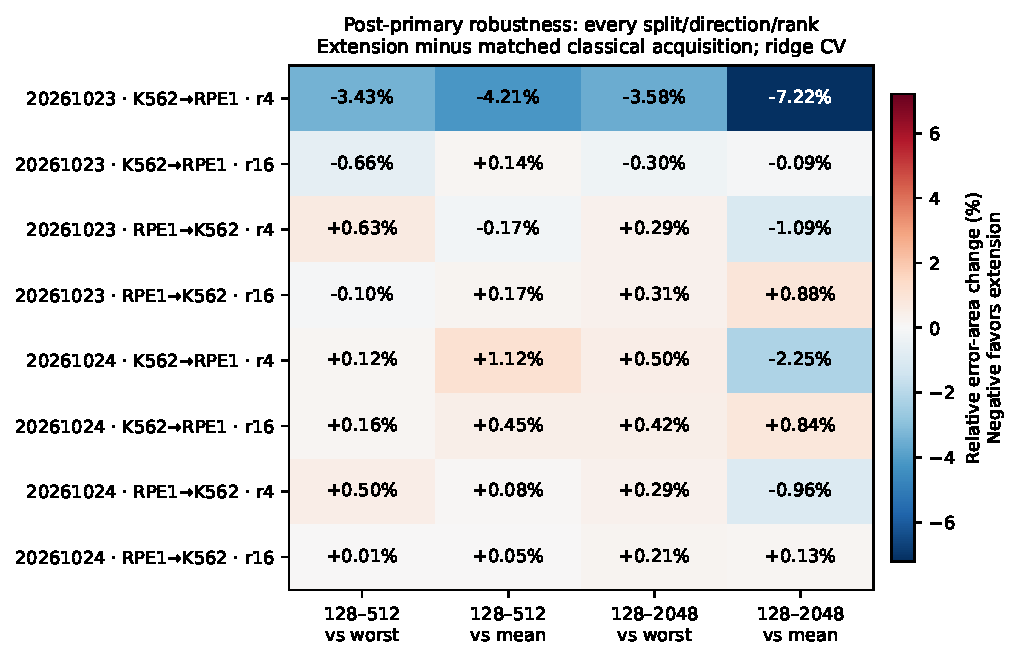
\includegraphics[width=\linewidth]{figures/robustness-matrix.pdf}
\caption{Every post-primary robustness cell. Percent changes use each reference's own error area; negative favors the fixed-RBF extension with the same paid-validation ridge predictor. The original subgrid uses 128/256/512 and the full grid adds 1,024/2,048. Colors and numbers are descriptive point estimates, not multiplicity-adjusted evidence or eight independent trials. Absolute paired differences and conditional query ranges are reported in the accompanying tables.}
\label{fig:robustness}
\end{figure}

\begin{table}[htbp]
\centering\footnotesize
\caption{All wider-grid robustness contrasts (128--2,048), in units $10^{-5}$. $\Delta_W$/$\Delta_M$ compare the extension with worst/mean query. Ranges are conditional query resampling, with three acquisition seeds averaged within query. Split 23/24 abbreviates 20261023/20261024. Negative favors the extension; no biological or multiple-comparison interpretation is assigned.}
\label{tab:robust-full}
\begin{tabular}{lrrrrrr}
\toprule
Direction & Split & Rank & $\Delta_W$ & Query range & $\Delta_M$ & Query range \\
\midrule
K562$\to$RPE1 & 23 & 4 & -30.174 & [-57.061, -5.193] & -63.181 & [-107.791, -22.524] \\
K562$\to$RPE1 & 23 & 16 & -2.644 & [-9.552, +5.503] & -0.807 & [-13.299, +11.646] \\
RPE1$\to$K562 & 23 & 4 & +1.605 & [-1.921, +6.252] & -6.104 & [-12.337, -0.916] \\
RPE1$\to$K562 & 23 & 16 & +1.730 & [+0.054, +3.295] & +4.929 & [+2.298, +7.684] \\
K562$\to$RPE1 & 24 & 4 & +3.562 & [-10.151, +17.193] & -16.525 & [-38.348, +3.963] \\
K562$\to$RPE1 & 24 & 16 & +3.192 & [-0.178, +6.982] & +6.404 & [-10.812, +24.471] \\
RPE1$\to$K562 & 24 & 4 & +1.628 & [-0.484, +4.344] & -5.407 & [-12.695, +0.485] \\
RPE1$\to$K562 & 24 & 16 & +1.198 & [+0.288, +2.279] & +0.717 & [+0.028, +1.528] \\
\bottomrule
\end{tabular}

\end{table}

Unlike rank four, rank 16 is estimated-unsupported for every query at budget 128, then fully supported from budget 256 onward for every policy and cell. This directly challenges the original already-supported regime. It still concerns estimated source coordinates, not oracle biological support. Extension/ridge selects zero in 9/60 rank-four and 10/60 rank-16 fits; at budget 128 this occurs in 8/12 fits for each rank. There are no extension null selections at 512, 1,024 or 2,048. The largest ridge penalty is selected in 9/60 and 30/60 fits, respectively. Support changes and shrinkage therefore coexist; a weak-prior acquisition variance remains distinct from actual prediction risk. Complete per-budget penalties, controls, opened identities and source-half shifts are retained.

These repeated episodes are dependent. Original--new query overlaps are 31/131 and 33/131; the two new splits share 35/131 queries. Within a direction all 50,912 source cells are shared. Across same-direction split pairs, acquisition banks overlap by 12,730--12,864 cells, query assessment by 316--363 and assessment controls by 121--131. In the opposite direction the supplied source includes all 4,448 cells used by the other task's scorer. Each task obeys its own declared information boundary, but this role reuse prevents treating the matrix as new untouched external validation. No pooling or subgroup selection converts these exploratory contrasts into a renewed primary result.

\begin{table}[htbp]
\centering\footnotesize
\caption{The same new robustness runs restricted to the 128--512 subgrid. Units, sign, split labels and conditional ranges match Table~\ref{tab:robust-full}. Three of eight point contrasts favor the extension against worst-query and two of eight against mean-query. All cells remain visible regardless of direction or sign.}
\label{tab:robust-original}
\begin{tabular}{lrrrrrr}
\toprule
Direction & Split & Rank & $\Delta_W$ & Query range & $\Delta_M$ & Query range \\
\midrule
K562$\to$RPE1 & 23 & 4 & -30.611 & [-60.093, -4.850] & -37.794 & [-69.811, -9.103] \\
K562$\to$RPE1 & 23 & 16 & -5.962 & [-10.975, -1.637] & +1.229 & [-4.039, +7.073] \\
RPE1$\to$K562 & 23 & 4 & +3.530 & [+0.439, +7.564] & -0.968 & [-2.040, -0.036] \\
RPE1$\to$K562 & 23 & 16 & -0.565 & [-1.142, -0.074] & +0.973 & [-0.204, +2.267] \\
K562$\to$RPE1 & 24 & 4 & +0.907 & [-13.166, +15.911] & +8.482 & [-11.522, +30.455] \\
K562$\to$RPE1 & 24 & 16 & +1.269 & [-0.500, +3.530] & +3.450 & [-5.814, +14.126] \\
RPE1$\to$K562 & 24 & 4 & +2.814 & [-0.282, +6.610] & +0.471 & [+0.189, +0.801] \\
RPE1$\to$K562 & 24 & 16 & +0.041 & [-0.035, +0.126] & +0.265 & [-0.103, +0.705] \\
\bottomrule
\end{tabular}

\end{table}

\section{Discussion}
The frozen experiment provides no demonstrated improvement from the evaluated fixed-kernel augmentation over worst-query acquisition. That conclusion is local: the post-primary matrix includes a forward rank-four split with a benefit on both budget grids, alongside six of eight point contrasts in the opposite direction. The evidence therefore supports sensitivity and limited reliability of this particular surrogate, rather than a general claim that discrepancy-aware design cannot help. This conditional success is scientifically relevant and remains in the main results despite departing from the original negative pattern.

Several mechanisms explain why a plausible variance term need not improve prediction. Acquisition assumes a weak $.01$ design prior, while the actual predictor can select strong shrinkage or zero. The kernel treats the linear trend as known, has fixed unit amplitude, and is not part of the prediction model. Its posterior variance neither estimates realized nonlinear discrepancy nor optimizes paid-validation ridge risk. Moreover, worst-query targets a maximum whereas the endpoint averages queries. A future comparison could fit discrepancy amplitude using only paid data and align the design criterion with predictive risk, but that would be a new method requiring its own development and frozen evaluation.

The support failure sharpens a separate limitation. Numerical span is necessary for unregularized linear estimability when coordinates are fixed and correct; it is not evidence that a biological intervention response can be transported. Source error can fill a missing direction with noise, and ridge can stabilize an extrapolation without identifying it. Our constructed counterexample and interval failures demonstrate these possibilities but do not measure their real-world frequency. Similarly, full support in the original pilot means its negative result cannot by itself judge acquisition's value during an identification transition.

In the original low-budget replay, a large assessment-noise component, low absolute-direction and ordinal scores, heterogeneous query effects and strong zero/shrinkage references limit practical signal. The new rank-four full-grid reductions versus zero are larger, particularly forward, but squared-error gains alone do not establish useful biological forecasts. The selected 525-target cohort, released gene panels and count-uniform pools restrict the population. Survival, capture, effector and time-point differences remain. Bidirectional and repeated-split replay reuse the same data, and no additional donor or biological replicate is manufactured by resampling. Conditional query, cell and technical-batch ranges answer different questions; none supplies an interval for generalization to new biological contexts. There is no equivalence margin, power argument for absence of benefit, or multiplicity-adjusted search for a winning subgroup.

The resource nevertheless permits precise questions that are often obscured by differing information access. Source data, development exposures, scorer resources and actual recipient purchases are accounted separately. Common backbones isolate allocation from prediction; shared-control covariance links depth and control decisions; all paired contributions and comparator combinations are retained. This auditability supports trust in the stated experiment, but engineering checks cannot substitute for a scientific effect or independent validation. The reconstructed neural comparator and hypothetical action prices further restrict comparisons with published methods and laboratory workflows.

For researchers considering this rule, the evidence does not justify adopting the fixed augmentation as a generally superior default. It motivates testing representation, split, budget and predictor alignment before a prospective campaign, with biological replication and feasible acquisition economics. The reusable result is a narrowly specified evaluation of conditional successes and failures, together with a source-error counterexample and an executable assessment framework.

\section*{Author and publication statements}
\paragraph{Contributions and correspondence.} Abdullah Hamza is the sole author, responsible for the study, interpretation and manuscript. Correspondence: \href{mailto:abdullah2hamza@gmail.com}{abdullah2hamza@gmail.com}. Affiliation: Independent Researcher.
\paragraph{Funding and competing interests.} The author reports no external funding and no competing interests.
\paragraph{Data and ethics.} This computational study reuses published, de-identified cell-line perturbation datasets from scPerturb/Zenodo record 13350497 under their original terms. No new participants, animals or wet-laboratory experiments were enrolled or conducted. This statement describes the present computational work and does not assert a new institutional ethics determination. Dataset checksums, inclusion rules and preprocessing provenance are supplied with the reproducibility materials.
\paragraph{Code and materials.} Original software is MIT licensed; this manuscript is CC BY 4.0. Third-party data and cited work retain their own licenses. The submission materials include the complete source code, locked environment, configurations, manageable retained results, figure/table generator and editable manuscript sources. Large raw/prepared data and prediction arrays are regenerated from pinned public data rather than redistributed. The GitHub repository \url{https://github.com/abdullah2hamza-blip/MLResearch} is private during preparation; the accompanying code archive is the reader-accessible submission artifact to deposit with the manuscript. No public repository or permanent code DOI is claimed at this stage.
\paragraph{AI assistance.} OpenAI Codex assisted with implementation, analysis, drafting and two automated internal review passes. These checks were not external human peer review. AI tools are not authors; the named human author retains responsibility for verifying the content, references and submission and for complying with the destination's disclosure policy. No pretrained perturbation-predictor weights were used in the reported replay.

\clearpage
\bibliographystyle{plainnat}
\bibliography{references}
\clearpage
\appendix
\section{Classical identities and their limits}
\label{app:math}
\subsection{Nuisance baseline and shared-control information}
For one response coordinate, write the independent raw treatment means as $m_i=\mu_0+x_i^\top\beta+\epsilon_i$, with $\operatorname{var}(\epsilon_i)=d_i$, and the control mean as $m_0=\mu_0+\epsilon_0$, with variance $c>0$. Taking contrasts $Y_i=m_i-m_0$ yields Equation~\ref{eq:cov}. This derivation assumes independence of treatment and control means; shared batch effects can violate it.

Let $w_i=1/d_i$, $w_0=1/c$, $W=w_0+\sum_iw_i$, $s=\sum_iw_ix_i$ and $\mu=s/W$. The raw-mean weighted information for the unknown baseline and response coefficients is
\begin{equation}
 \begin{pmatrix}W&s^\top\\s&\sum_iw_ix_ix_i^\top\end{pmatrix}.
\end{equation}
Eliminating the baseline by its Schur complement gives
\begin{align}
 M&=\sum_iw_ix_ix_i^\top-ss^\top/W\\
  &=\sum_iw_i(x_i-\mu)(x_i-\mu)^\top+w_0\mu\mu^\top=X^\top C^{-1}X.
\end{align}
The centered expression and a factored whitening solve are used numerically. The source-feature intercept is part of $\beta$; it differs from the raw control baseline $\mu_0$, whose feature is zero. Ridge penalizes all response coefficients, including the appended source intercept, but not this eliminated nuisance baseline.

Adding precision $t>0$ at feature $x$ updates information by
\begin{equation}
 M_{\rm new}=M+\frac{t}{1+t/W}(x-\mu)(x-\mu)^\top \quad(W>0).
\end{equation}
At the first weighted group with no previous observations, centered information is zero. Rank-one inverse/determinant identities accelerate the hypothetical action scores. Variance forecasts are held fixed while evaluating each candidate action and updated from newly purchased cells afterward. Thus a positive hypothetical gain does not imply monotonically decreasing realized prediction error.

\subsection{Estimability is conditional on the supplied coordinates}
With $c>0$ and finite positive $d_i$, $C$ is positive definite, so $\operatorname{range}(M)=\operatorname{row}(X)$. If $q$ is outside this space, choose $h\in\operatorname{null}(X)$ with $q^\top h\ne0$. Parameters $\beta$ and $\beta+th$ give identical expected calibration observations for every $t$, while their query means differ by $tq^\top h$. The query is therefore not estimable in this fixed-feature model. If $q$ lies in the space, its unregularized ideal variance is $q^\top M^+q$.

A ridge inverse exists even outside the space because its uniqueness is supplied by a penalty, not additional observations. Moreover, replacing latent coordinates by noisy estimated source features can change the apparent row space. A numerical full-rank certificate about those estimates is not a certificate about population transfer. The simulation's missing-direction example demonstrates this logical distinction under a controlled construction; it does not estimate how often that failure occurs in real screens.

\subsection{Paid validation with a shared noisy reference}
For held-out contrast $Y_i=\delta_i+\epsilon_i-\epsilon_0$ and linear predictor $\widehat\delta_i=a^\top Y_{-i}$, let $d_i=\operatorname{var}(\epsilon_i)$, $c=\operatorname{var}(\epsilon_0)$ and $u=\sum_j a_j$. Under fixed features, fixed coefficients $a$ and independent mean-zero noises,
\begin{align}
 E[(Y_i-a^\top Y_{-i})^2]
 &= (\delta_i-a^\top\delta_{-i})^2+d_i+\sum_j a_j^2d_j+c(1-u)^2,\\
 E[(\widehat\delta_i-\delta_i)^2]
 &= (\delta_i-a^\top\delta_{-i})^2+\sum_j a_j^2d_j+cu^2.
\end{align}
Consequently, subtracting $d_i+c$ and adding $2cu$ to the held-out squared residual has the second expectation. Averaging expression coordinates gives the implemented scalar score. The null candidate has $a=0$. This is a fixed-design known-variance identity; estimated variances and adaptive acquisition depend on the same observations, and selecting the minimum score adds selection effects. We do not assert unbiasedness of the full adaptive procedure or a prediction-interval guarantee.

\subsection{Paired errors preserve the common control}
For frozen predictions $p_A,p_B\in\mathbb R^G$ and assessment contrast $\widetilde\delta_i=\overline T_i-\overline T_0$,
\begin{equation}
 D_i=\frac{\|p_A\|^2-\|p_B\|^2}{G}
      -\frac{2(p_A-p_B)^\top\overline T_i}{G}
      +\frac{2(p_A-p_B)^\top\overline T_0}{G}.
\end{equation}
The unknown truth's quadratic term cancels. Averaging seeds and trapezoid weights produces one constant and one projection vector per query. Cell resampling then operates on these low-dimensional treatment/control projections without refitting. The same resampled controls must be used for every query. An independent control resample per query would discard cross-query covariance and can understate the control contribution.

For fixed queries and independent cells, the analytic mean-difference variance has treatment terms proportional to $\sum_i\operatorname{var}(t_i)/n_i$ and a control term $\operatorname{var}(\sum_i z_i)/n_0$, rather than $\sum_i\operatorname{var}(z_i)/n_0$. Implementation tests check this identity against direct resampling. Query resampling instead changes which empirical interventions receive weight while fixing their observed assessment contrasts. The two procedures have different scopes and are not a calibrated joint biological interval. Nearly singleton guide/batch strata and missing biological replication remain limitations, not problems solved by the algebra.

\section{Complete baseline rules and controlled data model}
\label{app:baselines}
\subsection{Additional allocation rules}
All actions are filtered by inventory, allowed action types and affordability before scoring. Deterministic score ties follow sorted action order; seeded order/random ties are explicit below. Every score is divided by the action's full cell/setup cost.

Random/equal allocation first buys controls when their accumulated cost is below the configured fraction of current spend, or when no treatment action remains. Otherwise it selects randomly among treatments at minimum current depth, including unopened interventions at depth zero. Fixed grid has the same control rule, then chooses the earliest seeded intervention below target depth (eight after development); if none remains, it chooses the earliest among minimum-depth ties. The primary configured control fraction is $.125$; the original controlled study uses $.25$.

Diversity is a hybrid: an unopened treatment scores its minimum squared source-feature distance to any opened treatment, an already opened treatment scores zero, and controls score the decrease in maximum working query variance. With no opened treatment it uses feature norm. D-optimal scores the increase in $\log\det(M+.01I)$. Reliability scores the decrease in one scalar mean variance: $v_0/n_0-v_0/(n_0+k)$ for $k$ controls, or $v_i/\max(n_i,1)-v_i/(n_i+k)$ for a treatment. It does not use a calibrated probability of transfer success.

Disagreement fits paid-data GLS at the full coordinate resolution and at the first $\max(1,\lfloor(r+1)/2\rfloor)$ features, including the intercept. Their ridge penalties are $.1$ and $10\max(.1,.01)=1$. Let $d_q$ be their mean squared prediction disagreement over genes, normalized by $\max(\overline d,10^{-8})$. The rule scores mean query-variance reduction weighted by $1+d_q$. Worst-query, mean-query, disagreement and the fixed-RBF rule add the same finite support bonus $10^6H$ while any query is unsupported; other heuristics do not. These are explicit benchmark heuristics, not reproductions of published acquisition algorithms.

The original external ablations set the discrepancy weight to zero or $.25$, fix intervention opening order to the seeded order, forbid extra depth, forbid extra controls, forbid new interventions after the pilot, or replace shared-control covariance in the acquisition score with diagonal effect variances. This last design ablation still uses the covariance-correct prediction backbone; it does not change the actual shared controls. Prohibitions apply after the common paid pilot. Fixed order restricts new openings, while allowed control/depth choices retain their action scores. The separate price study's identity-only ablation jointly forbids extra depth and extra controls.

\subsection{Additional prediction backbones}
Let $s_i\in\R^G$ be the supplied source effect and $y_i$ the purchased recipient contrast, for $i\in\mathcal A$. Zero predicts zero and source copy predicts $s_q$. Shared mean predicts $|\mathcal A|^{-1}\sum_i y_i$ for every query. Scalar affine adaptation pools all purchased intervention/gene pairs into ordinary least squares $y_{ig}=a+bs_{ig}$, with scalar slope and intercept, then predicts $a+bs_{qg}$; its source Gram denominator is floored at $10^{-12}$.

Fixed ridge uses GLS penalty $.1$; paid-validation ridge includes the stated penalty grid and zero candidate. The local residual heuristic predicts
\begin{equation}
 \widehat\delta_q=s_q+\frac{|\mathcal A|}{|\mathcal A|+4}
       \sum_{i\in\mathcal A}w_{qi}(y_i-s_i),\qquad
 w_{qi}\propto\frac{\exp[-\|z_q-z_i\|^2/(2r)]}{d_i+c+.1},
 \quad\sum_i w_{qi}=1.
\end{equation}
The weight denominator is protected numerically at $10^{-12}$. This is an explicitly heuristic adaptation, distinct from the reconstructed transport network in Appendix~\ref{app:implementation}. None of these predictors reads assessment outcomes for fitting or selection.

\subsection{Known-truth generative model}
Simulated continuous expression is used as provided, without count normalization. For each generated world draw 24 latent vectors $h_i\sim N(0,I_3)$, independently of a metadata-seeded six-query split. For calibration identities only, multiply the last latent coordinate by $a$. Draw independent loadings $L_S,L_T\in\R^{3\times64}$ and a nonlinear gene direction $u\in\R^{64}$ with iid $N(0,.3^2)$ entries. With independent $e_i\sim N(0,I_{64})$, define
\begin{align}
 s_i^*&=h_i^\top L_S,&s_i&=s_i^*+\tau e_i,\\
 \delta_i&=h_i^\top L_T+m\sin(h_{i1})u.
\end{align}
The source-feature offset $\tau e_i$ is persistent across all source cells of intervention $i$, unlike independent cell measurement noise. Each context has an independent baseline $\mu_c\sim N(0,.5^2I)$; source cells are $\mu_S+s_i+\sigma_S\epsilon$, recipient cells are $\mu_T+\delta_i+\sigma_T\epsilon$, and control cells omit the intervention effect. All $\epsilon$ are independent standard Gaussian vectors before optional batches. Recipient control SD is $\kappa\sigma_T$, while source control SD is $\sigma_S$. Float32 values enter the same episode/acquisition/scoring interface. Truth, including $s_i^*$ and $\delta_i$, stays outside policy objects.

Baseline parameters are $(a,\tau,m,\sigma_S,\sigma_T,\kappa)=(1,0,0,.5,1,1)$. Single-factor changes are $\tau=.5$ or 1; $\sigma_S=2$; $\sigma_T=.5$ or 2; $\kappa=4$ (control \emph{standard deviation}, hence variance times 16); and $m=2$. Missing-direction cases set $a=0$, with ordinary source noise $.5$ or exact source noise zero; an exact full-rank source case keeps $a=1$ and sets $\sigma_S=0$. Source-identity derangement and query-source gene permutation are separate controls.

The batch scenario adds one shared vector $b_j\sim N(0,I_{64})$ to each recipient cell assigned to one of four cyclic technical batches. Full recipient treatment/control conditions are balanced across batches, so the full-condition batch mean cancels in the truth contrast; smaller acquisition/assessment banks can be unbalanced. Batch vectors are shared across interventions, creating dependence. Source conditions contain 32 treatment cells and 128 controls; recipient conditions contain 48 treatment cells and 128 controls, split into the stated banks. The latent/data stream uses a seed sequence distinct from the metadata split stream. All scenarios reuse five world seeds as common random draws; independence is not multiplied by 14 scenario labels.

\section{Implementation, comparator fidelity and complete results}
\label{app:implementation}
\subsection{Operational settings and reproducibility}
The software is a typed CPU-first Python package with a locked dependency environment and command-line stages for verified downloads, H5AD audit, bounded-memory preprocessing, episodes, finite-pool acquisition, scoring and reporting. Dense/CSR inputs stream rows; CSC inputs stream columns and compute full-panel library totals before transformation. Float32 memory-mapped prepared arrays avoid loading a full dense atlas. Original and canonical gene/guide/context identifiers and unavailable batch/donor metadata remain explicit. The public episode exposes source summaries and inventory, while only the runner loads private recipient row maps.

Each prediction checkpoint binds its numeric artifact, exact ledger prefix, event count and spend. Joint suites archive acquisition manifests and authenticate every peer before opening any scorer. No source or declared configuration/evidence mutation is allowed during a live suite. A confirmed interrupted scoring phase may resume from its original gate; a timeout alone does not justify restarting acquisition. Historical source snapshots accompany every major stage. This is reproducibility and cooperative access control, not protection against an actor who rewrites all sources and hashes.

The original fixed grid was tuned only on development to control fraction $.125$ and depth 8. Classical design uses a $.01I$ weak design prior, independently of the predictor's fixed ridge $.1$ or paid-validation penalty. Source rank is four in the original real replay and three in the original controlled grid. Source half sensitivity refits ridge predictors on two source halves at fixed paid ledgers; it does not refit acquisition or neural models and is not a confidence bound. The source warning compares squared public source-response norm with twice estimated mean measurement variance; it has no calibrated deferral guarantee.

\subsection{The reconstructed transfer comparator}
The recipient-local network and transport reconstruction use the same paid observations. Source and recipient responses from training identities alone define an exact low-rank basis, capped at 16 and the available centered rank; validation and query source tokens are excluded from fitting that basis. Descriptors are correlations of the target gene with 64 variable genes in paid controls, augmented by mean, standard deviation and detection rate. A target gene absent from the released expression panel receives an explicit zero descriptor and a missingness flag, rather than free external measurements.

A LayerNorm/128-unit/GELU network predicts response coefficients. The NumPy AdamW implementation uses learning rate $.001$, weight decay $.0001$, batch 16 and three epochs per round, up to 100 rounds with patience 15. Model seed is 20261022 and paid identity split seed is 20260718; 20\% of paid identities are reserved for validation, with at least one validation identity and two training identities. An affine source-to-recipient expert selects ridge strength from $.001,.01,.1,1,10$, scaled by average per-coordinate source Gram energy. Interpolation to the local predictor is clipped to $[0,1]$ on that same paid validation set.

These choices differ from author-code reproduction: there is one source, exact train-only PCA instead of a covariance sketch, a declared optimizer and energy scale, explicitly missing descriptors, and a different cohort/budget regime from the original PerturbMap study \citep{perturbmap2026}. We report this comparator's performance, not reproduction or refutation of that article. Because early stopping, expert selection and interpolation reuse validation outcomes, positive fitted gain is not independent evidence that a route generalizes. Zero interpolation is feasible, so nonnegative fitted gain is partly enforced by optimization.

PI code review found a diagnostic error in the historical formula
\begin{equation}
 \rho=\max\{0,1-\mathrm{MSE}_{route}/(\mathrm{MSE}_{base}+10^{-12})\}.
\end{equation} For positive base error this is positive even at equal errors. Twenty of the original 720 checkpoints have $\alpha=0$ and equal route/base errors but were marked accepted. Their authenticated reconstruction and local-base arrays are byte-identical; the other 700 have strictly positive fitted gain and positive interpolation. Thus the correction changes those flags, not any original prediction score. Version 0.2.0 uses $\max(0,\mathrm{MSE}_{base}-\mathrm{MSE}_{route})/\max(\mathrm{MSE}_{base},10^{-12})$ and requires positive interpolation and positive gain. Edge-case tests include zero displacement, perfect base, an analytic fractional optimum, and an improvement too small to resolve beside a large squared error. Original artifacts remain unmodified, and the audit identifies every affected checkpoint.

\subsection{Full crossed primary prediction results}
Tables~\ref{tab:full-forward}--\ref{tab:full-reverse} report all original policy/backbone point estimates on the same fixed endpoint. They are descriptive complete comparisons, not a multiplicity-adjusted ranking of biological methods. The zero/copy columns have zero recipient measurement-use cost even though displayed next to each policy's counterfactual paid trajectory. ``Local'' denotes the recipient-local network and ``Recon.'' the qualified reconstruction. Appendix ablation labels refer to the fixed-RBF augmentation; predictions retain the same covariance-correct backbone. Tables~\ref{tab:all-scenarios} and \ref{tab:intervals} additionally report all original controlled scenarios and both nominal Gaussian diagnostic levels.

\begin{table}[p]
\centering\footnotesize
\caption{K562 to RPE1: full normalized MSE areas, multiplied by $10^3$. All five acquisition seeds and 128/256/512 budgets are included. Fixed ridge and paid-validation ridge (CV) are distinct. These data precede the gate diagnostic correction, which leaves predictions unchanged.}
\label{tab:full-forward}
\begin{tabular}{lrrrrrrrrr}
\toprule
Policy & Zero & Mean & Copy & Affine & Ridge & CV & Residual & Local & Recon. \\
\midrule
Random/equal & 8.125 & 12.588 & 9.029 & 7.859 & 39.220 & 8.032 & 11.585 & 10.201 & 11.060 \\
Fixed grid & 8.125 & 12.749 & 9.029 & 7.937 & 45.785 & 8.082 & 11.614 & 10.072 & 11.246 \\
Diversity & 8.125 & 17.695 & 9.029 & 8.179 & 18.653 & 7.707 & 13.845 & 11.910 & 14.273 \\
D-optimal & 8.125 & 14.681 & 9.029 & 8.138 & 16.885 & 7.763 & 11.738 & 10.880 & 12.397 \\
Worst query & 8.125 & 13.012 & 9.029 & 8.009 & 16.558 & 7.824 & 11.396 & 10.504 & 11.077 \\
Mean query & 8.125 & 12.080 & 9.029 & 8.017 & 13.687 & 7.806 & 10.724 & 9.805 & 10.270 \\
Reliability & 8.125 & 19.933 & 9.029 & 8.054 & 27.219 & 7.737 & 15.173 & 13.400 & 16.352 \\
Disagreement & 8.125 & 12.356 & 9.029 & 7.984 & 13.946 & 7.796 & 11.038 & 9.575 & 10.302 \\
RBF aug. & 8.125 & 14.139 & 9.029 & 7.996 & 17.531 & 7.868 & 12.220 & 10.142 & 11.676 \\
RBF weight .25 & 8.125 & 13.579 & 9.029 & 7.974 & 16.898 & 7.852 & 11.842 & 10.342 & 11.447 \\
No extra depth & 8.125 & 13.542 & 9.029 & 8.015 & 17.424 & 7.824 & 11.883 & 9.962 & 11.462 \\
Fixed controls & 8.125 & 17.328 & 9.029 & 7.951 & 20.680 & 7.893 & 14.725 & 11.583 & 15.234 \\
No openings & 8.125 & 14.700 & 9.029 & 7.922 & 408.023 & 8.285 & 11.004 & 11.729 & 12.578 \\
Fixed order & 8.125 & 15.525 & 9.029 & 7.941 & 94.800 & 8.385 & 11.694 & 12.113 & 13.323 \\
Diagonal noise & 8.125 & 14.916 & 9.029 & 8.018 & 18.245 & 7.858 & 12.806 & 10.901 & 12.651 \\
RBF weight 0 & 8.125 & 13.012 & 9.029 & 8.009 & 16.558 & 7.824 & 11.396 & 10.504 & 11.077 \\
\bottomrule
\end{tabular}

\end{table}
\begin{table}[p]
\centering\footnotesize
\caption{RPE1 to K562: full normalized MSE areas, multiplied by $10^3$, under the same endpoint and qualifications as Table~\ref{tab:full-forward}. Directions reuse observations and are reported separately.}
\label{tab:full-reverse}
\begin{tabular}{lrrrrrrrrr}
\toprule
Policy & Zero & Mean & Copy & Affine & Ridge & CV & Residual & Local & Recon. \\
\midrule
Random/equal & 5.760 & 10.581 & 8.942 & 5.678 & 40.214 & 5.755 & 11.224 & 8.196 & 9.303 \\
Fixed grid & 5.760 & 10.545 & 8.942 & 5.714 & 40.994 & 5.760 & 11.190 & 8.325 & 9.496 \\
Diversity & 5.760 & 13.012 & 8.942 & 5.775 & 15.933 & 5.745 & 13.647 & 10.883 & 12.201 \\
D-optimal & 5.760 & 10.718 & 8.942 & 5.718 & 12.915 & 5.742 & 11.304 & 9.390 & 10.072 \\
Worst query & 5.760 & 10.316 & 8.942 & 5.687 & 16.002 & 5.723 & 11.105 & 8.732 & 9.816 \\
Mean query & 5.760 & 8.948 & 8.942 & 5.625 & 10.755 & 5.751 & 10.011 & 8.128 & 8.342 \\
Reliability & 5.760 & 15.148 & 8.942 & 5.798 & 26.054 & 5.760 & 14.958 & 11.704 & 13.862 \\
Disagreement & 5.760 & 9.214 & 8.942 & 5.650 & 11.027 & 5.736 & 10.176 & 8.642 & 8.644 \\
RBF aug. & 5.760 & 11.351 & 8.942 & 5.685 & 16.967 & 5.724 & 11.816 & 8.823 & 10.228 \\
RBF weight .25 & 5.760 & 10.606 & 8.942 & 5.681 & 16.180 & 5.721 & 11.267 & 8.711 & 9.544 \\
No extra depth & 5.760 & 10.592 & 8.942 & 5.683 & 16.388 & 5.731 & 11.324 & 8.557 & 9.794 \\
Fixed controls & 5.760 & 14.810 & 8.942 & 5.763 & 20.138 & 5.723 & 14.438 & 10.601 & 13.416 \\
No openings & 5.760 & 11.544 & 8.942 & 5.728 & 215.028 & 5.762 & 10.379 & 9.507 & 10.472 \\
Fixed order & 5.760 & 12.873 & 8.942 & 5.784 & 64.430 & 5.762 & 11.412 & 10.560 & 11.675 \\
Diagonal noise & 5.760 & 11.925 & 8.942 & 5.709 & 17.453 & 5.724 & 12.240 & 9.270 & 11.170 \\
RBF weight 0 & 5.760 & 10.316 & 8.942 & 5.687 & 16.002 & 5.723 & 11.105 & 8.732 & 9.816 \\
\bottomrule
\end{tabular}

\end{table}

\begin{table}[p]
\centering\footnotesize
\caption{All 14 original controlled scenarios: extension/ridge-CV true-error area $A_E$, paired difference from worst-query, Monte Carlo standard error of the paired difference, and relative change. Negative differences favor the extension. Each row uses five generated worlds, averaging six queries and five acquisition seeds within each world. Scenarios share random draws and are not independent replications. These settings use discrepancy weight $.25$.}
\label{tab:all-scenarios}
\begin{tabular}{lrrrr}
\toprule
Scenario & $A_E$ & $\Delta$ & MC SE($\Delta$) & Change (\%) \\
\midrule
Baseline & 0.05228 & +0.00073 & 0.00045 & +1.411 \\
Shared batches & 0.06703 & +0.00192 & 0.00128 & +2.951 \\
Control SD x4 & 0.06780 & +0.00034 & 0.00063 & +0.503 \\
Full rank, exact source & 0.05157 & +0.00043 & 0.00060 & +0.843 \\
Missing direction, exact & 0.14578 & +0.00022 & 0.00047 & +0.155 \\
Nonlinear shift & 0.09307 & -0.00498 & 0.00121 & -5.084 \\
Query genes shuffled & 0.30467 & +0.00080 & 0.00036 & +0.263 \\
Missing direction, noisy & 0.18595 & +0.00024 & 0.00024 & +0.131 \\
Recipient noise SD 2 & 0.10345 & -0.00177 & 0.00203 & -1.682 \\
Recipient noise SD .5 & 0.02030 & +0.00116 & 0.00030 & +6.047 \\
Source error SD .5 & 0.06985 & -0.00006 & 0.00080 & -0.090 \\
Source error SD 1 & 0.13242 & -0.00423 & 0.00193 & -3.098 \\
Source identity shuffled & 0.25768 & +0.00120 & 0.00304 & +0.468 \\
Source noise SD 2 & 0.06158 & +0.00206 & 0.00068 & +3.465 \\
\bottomrule
\end{tabular}

\end{table}

\begin{table}[p]
\centering\footnotesize
\caption{Known-truth Gaussian diagnostics at budget 192 for fixed ridge/worst-query. Entries are mean coordinate coverage and full width, conditional on finite intervals. ``Finite'' counts query/seed intervals across five worlds (six queries and five acquisition seeds each); these 150 observations are not independent biological replicates. The exact-source missing-direction case has no finite interval. The original full tables retain every scenario and checkpoint. Neither nominal level is a validated adaptive inference procedure.}
\label{tab:intervals}
\begin{tabular}{lrrrrr}
\toprule
Scenario & 90\% & 95\% & Width90 & Width95 & Finite \\
\midrule
Baseline & 0.9091 & 0.9540 & 0.7530 & 0.8973 & 150/150 \\
Nonlinear shift & 0.8025 & 0.8635 & 0.7530 & 0.8973 & 150/150 \\
Source error SD 1 & 0.7005 & 0.7814 & 0.7285 & 0.8680 & 150/150 \\
Shared batches & 0.9380 & 0.9726 & 0.9876 & 1.1768 & 150/150 \\
Missing direction, noisy & 0.9298 & 0.9671 & 5.2968 & 6.3117 & 150/150 \\
Missing direction, exact & Undefined & Undefined & Undefined & Undefined & 0/150 \\
\bottomrule
\end{tabular}

\end{table}

\section{Assessment scopes, cost sensitivity and stronger-information reference}
\label{app:assessment}
\subsection{Separate uncertainty questions}
Table~\ref{tab:uncertainty} reports four scopes for the same original paired endpoint. The query range can cross zero even when fixed-query cell or batch ranges do not: their randomization units and conditioning differ. All procedures preserve the shared assessment controls. They omit uncertainty in source estimation, model selection and prospective biological contexts.

\begin{table}[htbp]
\centering\small
\caption{Original extension minus worst-query area: central 95\% resampling ranges in units $10^{-5}$. The point estimates remain $4.4212$ forward and $.0789$ reverse. Each row answers its own conditional question; no row supplies biological replication or a joint interval.}
\label{tab:uncertainty}
\begin{tabular}{llr}
\toprule
Direction & Scope & Conditional range \\
\midrule
K562$\to$RPE1 & Queries; fixed bank & [-4.4957, +13.0315] \\
K562$\to$RPE1 & Cells; fixed queries & [+2.6568, +6.1010] \\
K562$\to$RPE1 & Stratified cells & [+3.6524, +5.1900] \\
K562$\to$RPE1 & Technical-batch weights & [+2.9794, +5.9697] \\
RPE1$\to$K562 & Queries; fixed bank & [-0.4150, +0.5948] \\
RPE1$\to$K562 & Cells; fixed queries & [-0.1554, +0.3173] \\
RPE1$\to$K562 & Stratified cells & [-0.0070, +0.1617] \\
RPE1$\to$K562 & Technical-batch weights & [-0.1356, +0.2770] \\
\bottomrule
\end{tabular}

\end{table}

Guide/batch stratification is severely limited by sparse strata: 243/256 forward and 247/256 reverse assessment controls are in singleton strata, as are 2,558/4,192 and 2,328/4,192 treatment cells. A singleton cannot exhibit within-stratum resampling variation. Technical-batch reweighting changes the weights of observed batches; it does not introduce new biological replicates. The analytic independent-cell projection variance is a numerical cross-check, not evidence that real cells satisfy independence.

\subsection{Absolute error and ordinal denominators}
\begin{table}[htbp]
\centering\small
\caption{Budget-512 diagnostics on original extension purchases. MSE uses units $10^{-3}$. Rank is the fixed-gene Spearman score across query identities; ``Permuted'' uses one fixed scoring-coordinate permutation shared across query rows, without refitting. ``Defined'' is the fraction of 36,130 gene/seed correlations that are defined; undefined terms contribute neutral zero to the fixed-gene aggregate. Zero is a zero-recipient-cost reference even when tabulated beside purchased predictors. All 131 queries and 7,226 aligned genes are retained.}
\label{tab:ranking}
\begin{tabular}{llrrrr}
\toprule
Direction & Predictor & MSE & Rank score & Permuted & Defined \\
\midrule
K562$\to$RPE1 & Zero & 8.1251 & 0.00000 & 0.00000 & 0.00 \\
K562$\to$RPE1 & Source copy & 9.0291 & 0.07335 & 0.01218 & 1.00 \\
K562$\to$RPE1 & Paid ridge & 7.7147 & 0.07931 & 0.00791 & 1.00 \\
K562$\to$RPE1 & Local network & 9.0965 & 0.01527 & 0.00332 & 1.00 \\
K562$\to$RPE1 & Reconstruction & 9.8443 & 0.09087 & 0.01579 & 1.00 \\
RPE1$\to$K562 & Zero & 5.7597 & 0.00000 & 0.00000 & 0.00 \\
RPE1$\to$K562 & Source copy & 8.9425 & 0.06820 & 0.00803 & 1.00 \\
RPE1$\to$K562 & Paid ridge & 5.6789 & 0.03856 & 0.00207 & 1.00 \\
RPE1$\to$K562 & Local network & 7.7433 & -0.00212 & -0.00083 & 1.00 \\
RPE1$\to$K562 & Reconstruction & 7.6081 & 0.03903 & 0.00300 & 1.00 \\
\bottomrule
\end{tabular}

\end{table}

The retained ranking tables also report the mean over defined genes, undefined counts, sign-tie rules, raw/centered cosines and within-query gene correlations. These distinct estimands should not be interchanged. Across-query gene ranks are invariant to a per-gene common control shift; absolute effects are not.

\subsection{Setup price and finite-pool exhaustion}
At setup price zero, every unconstrained policy exhausts the 496-unit acquisition inventory before the first nominal budget of 512; the combined identity-only ablation spends 160. Equal final predictions among the unconstrained policies are mechanically uninformative about acquisition quality. At setup price 16, the available inventory is 784 and the identity-only limit is 448. At setup price 64, unconstrained policies reach the final 1,024 budget, while constrained variants may underspend earlier. These are finite inventory effects, not refunds or hidden reassignment of observations.

Extension/worst-query true-error area changes at setup price 16 are $+1.383\%$ in baseline and $+1.474\%$ with nonlinear shift; at price 64 they are $+1.248\%$ and $-.704\%$. Price-zero changes are exactly zero after exhaustion. Each comparison averages five generated worlds and five acquisition seeds, with worlds shared across prices/scenarios. The unchanged $.25$ discrepancy weight and larger budgets differ from the primary external configuration. Full spend curves, world-level differences and identity-only results accompany the release.

\subsection{Direct query measurement}
The stronger-information reference directly buys reserved query cells and controls, using different cell-order seeds and an independent scorer. With 131 queries, setup price four, depths 2, 4, 8, 16, 32 and 64 and matched control increments, actual costs are 802, 1,064, 1,588, 2,684, 4,844 and 9,164. At the smallest/largest depths mean MSE is $.08181/.00755$ forward and $.07791/.00716$ reverse. Small direct samples are noisy; these are raw direct contrasts, not an optimized estimator for all procedures allowed query information.

Its minimum cost exceeds the original primary maximum of 512. The later robustness grid extends into the same cost range but has no exactly matched checkpoint/task comparison. We therefore infer neither a universal crossover budget nor laboratory savings. All 60 direct predictions and ledger prefixes reproduce byte-for-byte on re-execution. This verifies the declared reference implementation, not experimental economics.

\section{Reproduction materials and computational scope}
\label{app:reproduction}
The accompanying source archive contains the article, bibliography, generated numerical tables, vector figures and a compiler helper. The code/evidence archive additionally contains Python sources, tests, configurations, locked dependencies, frozen historical code snapshots, audit records, compressed metric/ledger summaries and the table/figure generators. Machine-specific caches, credentials, raw expression matrices and large prediction arrays are excluded. Historical protocols remain intact; dated clarifications distinguish corrected descriptions and post-primary work.

\paragraph{Two reproduction levels.} A lightweight path authenticates the retained small evidence and regenerates manuscript tables/figures without expression data. A full path downloads the three checksum-pinned public H5AD files, rebuilds bounded-memory prepared arrays and episodes, acquires all predictions behind their joint freeze, then scores and re-analyzes. Source, configuration and episode hashes must match the corresponding historical run. Original predictions used version 0.1.0; the new robustness suite uses 0.2.0. The latter's gate correction changes embedded diagnostics in some original reconstructions, so a current-version rerun is not claimed to reproduce historical NPZ bytes merely because numerical prediction arrays agree. The release instructions identify the correct source snapshots.

\paragraph{Actual preparation checks.} All three full raw preparations were repeated, comparing 2,405,927,872 float32 values and all retained metadata byte-for-byte; 166,118 selected rows were reproduced. This is a full preprocessing check, not a second execution of every original acquisition experiment. Original primary and secondary artifact indexes authenticate their retained inputs. The additional robustness suite authenticates all 360 checkpoint predictions and 72 paid ledgers before scoring. Separate summaries preserve overlap and source-half diagnostics.

\paragraph{Environment and resources.} The original numerical studies used Python 3.12, locked NumPy/SciPy/HDF5 dependencies, one numerical worker and one BLAS thread on a local CPU. The hosted Kaggle notebook separately re-analyzes retained results; it is not a repeat of the original full-data experiments. No paid cloud computation or external perturbation-predictor weights are required. The original primary execution record reports 2,297.23 process-CPU seconds and 30,223.79 elapsed seconds with observed event gaps, so elapsed time should not be interpreted as uninterrupted computational cost. Its observed peak working set is 707,694,592 bytes. The additional robustness suite's observed peak working set is 790,515,712 bytes; it records elapsed acquisition/scoring times but has no comparable process-CPU counter. These are machine/run observations, not complexity or algorithm-speed claims. A standalone direct-reference reproduction used 37.09 elapsed and 22.91 CPU seconds.

\paragraph{Verification limits.} Automated numerical, covariance, accounting, leakage and resume checks, source and ledger authentication and internal mathematical reviews support the declared implementation. They cannot prove correctness against every software defect or validity of the transfer model. The release provides a requirement-by-requirement audit and instructions for clean installation, evidence verification, full-data replay and manuscript compilation, allowing readers to inspect the claims at their appropriate scope.

\end{document}
